\documentclass[12pt]{article}

% sbc template
\usepackage{sbc-template}
\usepackage{graphicx,url}
\usepackage[utf8]{inputenc}

% equations
\usepackage{amsmath}
\usepackage{multicol}
\usepackage[version=4]{mhchem}

% code snippets
\usepackage{graphicx}
\usepackage{listings}
\usepackage{xcolor}

% utils
\usepackage{lipsum}

%subfigures
\usepackage{caption}
\usepackage{subcaption}

% gro language definition
\definecolor{COLOR_COMMENTS}{RGB}{16, 97, 35}
\definecolor{COLOR_BACKGROUND}{rgb}{0.95,0.95,0.92}
\lstdefinelanguage{GROLANG}{
  morekeywords    =   {include,program,rate,ecoli},
  sensitive       =   false,
  morecomment     =   [l]{//},
  morestring      =   [b]",
}
\lstdefinestyle{GROSRC}
{
  language          =   GROLANG,
  basicstyle        =   \footnotesize,
  commentstyle      =   \color{COLOR_COMMENTS},
  backgroundcolor   =   \color{COLOR_BACKGROUND},
  frame             =   single,
  caption           =   Dummy gro file.,
  tabsize           =   4,
  numbers           =   left,
  framesep          =   25pt,
  xleftmargin       =   25pt,
  xrightmargin      =   25pt,
}

% parsed.intermediate style definition
\lstdefinestyle{INTERMEDIATE}{
  basicstyle        =   \footnotesize,
  backgroundcolor   =   \color{COLOR_BACKGROUND},
  caption           =   Compiled dummy.,
  framesep          =   25pt,
  xleftmargin       =   25pt,
  xrightmargin      =   25pt,
}

% output.xml style definiton
\lstdefinestyle{SBML}{
    language        =   XML,
    basicstyle      =   \tiny,
    caption         =   Final SBML document.,
}

% header info
\sloppy
\title{Albi:\\ A Gro compiler to the SBML standard}
\author{Alek Frohlich\inst{1}, Gustavo Biage\inst{1}}
\address{Departamento de Informatica e Estatística – Universidade Federal de Santa Catarina \\
Florianopolis – SC – Brazil
  \email{\{alek.frohlich,gustavo.c.biage\}@grad.ufsc.br}
}

% paper
\begin{document}
\maketitle

%       => the Growth of the area leads to the development of multicellular devices
%       => gro is well suited for this purpose
%       => however it isn't ready for compatibility
%       => introduce the objective of making it compatible
\begin{abstract}


    The growth of research areas such as synthetic biology and systems biology leads to an increased tendency to develop larger mathematical models to describe complex biological behavior. In order to enable natural flow of development of those models, scientists must have access to tools which increase the level of abstraction and enable reuse of biological components. The present work tackles those two problems by interfacing the existing programming language gro with SBML for model interchangeability and ease of model representation.


\end{abstract}

%       => what does albi fix that libSBML does not?
%       => what are the reasons we chose Gro as albi's primary language?
%       => what are the disadvantages of the Gro simulator
%       => what are the advantages of having the SBML model for a Gro program?
%       => introduce following sections
\section{Introduction}

    % virgula apos does not help much
    % gro minusculo!
    Even though a Systems Biology Markup Language API library (LibSBML) has already been developed \cite{Bornstein2008}, it only ought to be useful in cases where a new model is to be developed. In cases where there is a preexisting model, the availability of an SBML library does not help much since the previous model would have to be entirely rewritten to fit the API. Instead, the present work proposes a language parser that generates SBML code from previously built Gro models. gro is a language for programming, modeling, specifying and simulating the behavior of cells in growing micro colonies of microorganisms \cite{Jang2012}. The parser has been built upon it considering gro has many interesting syntactical constructs such as rate statements, program definitions and bacterial instantiation which can be expressed, respectively, as reactions, local name spaces and compartments in SBML documents.
    
    In regards to language support, gro is still tightly coupled with it's original simulator. Although the simulator has recently undergone big improvements in the sense that simulations behave more realistically \cite{Gutirrez2017}, it doesn't change the fact that using it is the only available way to validate gro models. This hinders the reproducibility of experiments built with the language. SBML models, on the other hand, are supported by more than 100 software systems \cite{Hucka2007}, making them more likely to be verified and reused.
    
    % researches vs researches
    If gro code were translated into SBML, the document could be further preserved as an entry in BioModels. BioModels is a database of curated SBML and CellML models maintained intended to provide researches with models related to a particular disease, biological process or molecular complex \cite{LeNovere2006}. Having a model curated is an even stronger guarantee of trustworthiness since the process is done manually for each model: Newly submitted models go through a series of syntactical analysis to confirm that they are valid and well formatted; The model is then numerically verified against the results claimed by the authoring paper; Finally, the validated model gets manually annotated and cross-linked to facilitate later search for it \cite{LeNovere2006}.
    
    The rest of the paper is structured as follows: In Sect. 2, we introduce the language parser and explain the process of converting gro files to SBML models from start to finish; In Sect. 3, we compile a Gro implementation of the repressilator, a synthetic delay oscillator, to equivalent SBML and then simulate it on COPASI, a pathway simulator \cite{Hoops2006}; In Sect. 4, we summarize what has been done and compare it with goals laid out at the start; In Sect. 5 we conclude by presenting possible extensions of the current work.
    

%       => compilation steps
\section{Architecture}

    
    The compilation process is divided in three steps: First, the code is validated, that is, it's checked against syntax errors such as missing semicolon in rate statements and semantic error such as using undeclared variables; Then the code gets compiled to Antimony, a modular model definition language \cite{Smith2009}; This format guides Tellurium in building the final SBML document. As we'll see in the following subsections, Tellurium makes use of the aforementioned libSBML API for code generation purposes.


%       => present Albi's syntax
%       => compiling gro source code
%       => explain renaming of variables according to program name space
%       => reduction of arithmetic expressions and parameter passing
%       => var, compartment, specie and const
\subsection{The parser}
    
    Currently, the parser only recognizes a subset of gro's syntax. Valid programs are constituted by global variable declarations, program definitions and E. coli instantiations. Parameters, messages and guarded statements are also recognized as valid syntax, however no semantic value is assigned to them given that control statements and user interaction do not make sense in the context of an SBML model. Below is an example of gro code containing the syntactical constructs just described.
    
    % dummy gro source code
    \begin{lstlisting}[style=GROSRC, caption=Example gro code.]
 include gro

 program prog() := {
     E := 25;
     F := 75 + E;
     K := 2 + F + E;
     rate(K) : { E := E + 1, F := F - 1 };
 };

 program dupl(X) := {
     E := 25 + X;
     F := 75 + E;
     K := 2 + F + E;
     rate(K*40) : { E := E + 1, F := F - 1 };
 };

 ecoli([], program prog() + dupl(10));
 ecoli([], program prog());
\end{lstlisting}
    
    % reforcar o antimony
    Compiling this file gives us \textit{parsed.intermediate}, the input file for Tellurium. As we can see, the compiler properly reduced arithmetic expressions and parameter passing. The compiler also renamed symbols declared inside program definitions to avoid name space clashes between multiple programs instantiated in the same compartment. If this renaming hadn't been done, there wouldn't be a way to differentiate the symbol E, whose name space is limited to reactions inside of prog, from the symbol E which was declared inside of dupl.
    
    ADICOES DO BIAGE AQUI ADICOES DO BIAGE AQUI ADICOES DO BIAGE AQUI ADICOES DO BIAGE AQUI ADICOES DO BIAGE AQUI ADICOES DO BIAGE AQUI ADICOES DO BIAGE AQUI ADICOES DO BIAGE AQUI ADICOES DO BIAGE AQUI ADICOES DO BIAGE AQUI
    
    % compiled dummy source code
    \input{example_compiled.tex}
    
\subsection{The Tellurium framework}

    Tellurium is a Python-based modeling environment for systems and synthetic biology \cite{Choi2018}. It aggregates multiple preexisting libraries such as libSBML, libAntimony and libSBOL to provide the modelling community access to an integrated modelling environment. Tellurium is organized in three functional pillars: Standards support, modelling support and utilities. We made extensive use of the libAntimony integration provided by standard support to build our SBML documents.


\section{Study case: The Repressilator}

    % passo-a-passo
    % ultima frase
    The goal of this experiment was to illustrate the proposed gro to SBML conversion scheme and so the experiment was conducted as follows: We first simulated the gro model for a well-known biological device, the Repressilator, in gro's built-in simulator; We Then compiled the source code down to SBML following the steps shown in Sect. 2; Finally we simulated the compiled gro code, an SBML document, in COPASI. Both simulations were done with the same initial conditions. We also demonstrated the the second simulation multiple times, each with a different simulation method to show the hinted gain of flexibility, as the built-in simulator is limited to one method, while COPASI clearly is not.


\subsection{Mathematical Model}

    \begin{figure}[h]
        \centering
        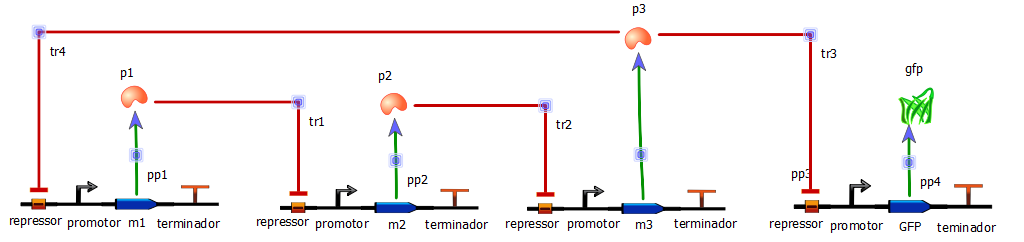
\includegraphics[scale = 0.7]{repressilator_model.png}
        \caption{Repressilator's genetic regulatory network.}
        \label{fig:repressilator_model}
    \end{figure}
    
    The Repressilator is a genetic regulatory network constituted by stitching together promoter-repressor pairs. It was first conceptualized by \cite{Elowitz2000}, who used the genes LacI and letR from E. coli and cI from phage lambda to build a three-repressor scheme. As illustrated in Figure~\ref{fig:repressilator_model}, the Repressilator works based on the fact that each gene expresses a protein which represses the next gene in the loop, meaning that a constituent gene in high concentration represses itself indirectly, leading to oscillatory behavior. In the original experiment, there was another biological component involved: the reporter, a green fluorescent protein (GFP) producing gene. It was used to visualize the network's oscillation.
    
    \begin{equation}
    \begin{aligned}[c]
        \frac{dm_{1}(t)}{dt} & = \alpha_{0} + \frac{\alpha}{1 + p_{3}(t)^{n}} - m_{1}(t) & \\
        \frac{dm_{2}(t)}{dt} & = \alpha_{0} + \frac{\alpha}{1 + p_{1}(t)^{n}} - m_{2}(t) & \\
        \frac{dm_{3}(t)}{dt} & = \alpha_{0} + \frac{\alpha}{1 + p_{2}(t)^{n}} - m_{3}(t) &
    \end{aligned}
    \begin{aligned}[c]
        \frac{dp_{1}(t)}{dt} & = \beta \cdot m_{1}(t) - \beta \cdot p_{1}(t) \\
        \frac{dp_{2}(t)}{dt} & = \beta \cdot m_{2}(t) - \beta \cdot p_{2}(t) \\
        \frac{dp_{3}(t)}{dt} & = \beta \cdot m_{3}(t) - \beta \cdot p_{3}(t)
    \end{aligned}
    \end{equation}

    As shown in \cite{Elowitz2000}, the high-level model from Figure~\ref{fig:repressilator_model} could also be presented as the above system of Ordinary Differential Equations (ODE). With that system of equations, we then built the corresponding gro model. The process was simple as we just separated the reactions from the equations, meaning, for example, that $\alpha_{0}$ from the left equations became the open reaction:
    
    \begin{equation}
    \ce{ ->[\alpha_{0}] m_{1} + m_{2} + m_{3}}
    \end{equation}
    
    On repeating this process for each ODE, we ended up with a total of 7 reactions, from which the new ones are listed below:
    
    % são todas abertas?
    \begin{equation}
    \begin{aligned}[c]
        \ce{ <=>[\alpha/(1 + p_{3}^n)][m_{1}] m_{1}} & & \\
        \ce{ <=>[\alpha/(1 + p_{1}^n)][m_{2}] m_{2}} & & \\
        \ce{ <=>[\alpha/(1 + p_{2}^n)][m_{3}] m_{3}} & &
    \end{aligned}
    \begin{aligned}[c]
        \ce{ <=>[\beta*m_{1}][\beta*p_{1}] p_{1}} \\
        \ce{ <=>[\beta*m_{2}][\beta*p_{2}] p_{2}} \\
        \ce{ <=>[\beta*m_{3}][\beta*p_{3}] p_{3}}
    \end{aligned}
    \end{equation}
    
    Which led us to the development of the following gro code:
    
    % repressilator source code
    \begin{lstlisting}[style=GROSRC]
 rate(alfa0) : { m1 := m1 + 1, m2 := m2 + 1, m3 := m3 + 1 };
 rate(alfa / (1 + p3^n)) : {m1 := m1 + 1};
 rate(m1) : {m1 := m1 - 1};
 rate(alfa / (1 + p1^n)) : {m2 := m2 + 1};
 rate(m2) : {m2 := m2 - 1};
 rate(alfa / (1 + p2^n)) : {m3 := m3 + 1};
 rate(m3) : {m3 := m3 - 1};
 rate(beta*m1) : {p1 := p1 + 1};
 rate(beta*p1) : {p1 := p1 - 1};
 rate(beta*m2) : {p2 := p2 + 1};
 rate(beta*p2) : {p2 := p2 - 1};
 rate(beta*m3) : {p3 := p3 + 1};
 rate(beta*p3) : {p3 := p3 - 1};
\end{lstlisting}

\subsection{Extracting behavior from Gro}
% MOVE PARA PROXIMA SUBSECAO
% In the process of obtaining the the oscillatory comportment, it is needed to establish a bi-stability, the information obtained is the manners of concentrations rapidly changing from a high "voltage" to a low "voltage", in the computer science perspective, which in this case the binary states are defined by the protein and molecules level of concentration. The initial concentrations values for this model is $m_{1} = m_{2} = m_{3} = 0$, $p1 = 0$, $p_{2} = 5$ and $p_{3} = 15$; the parameters are $n = 2$, $\alpha = 298.2$, $\alpha_{0} = 0.03$ and $\beta = 0.2$, of the same nature as the ones accomplished in the simulation graphs. \cite{ingalls2013mathematical}.
% \begin{figure}[h]
%     \centering
%     \includegraphics[scale = 0.5]{apagar.png}
%     \caption{Caption}
%     \label{fig:phase_plane_repressilator}
% \end{figure}
% When using deterministic simulations for a mathematical model in a hard to predict experiment, depending on how sensible to variables changes the model is, it can have a different performance than the one expected.\cite{Hahl2016} Stochastic simulations take in consideration that reactions occur randomly accordingly to their rate, this happens because intracellular concentration normally does not represent high values, there is a probability of odd behaviour, which should be accounted for.\cite{Bratsun2005}

% The repressilator, in particular, oscillation occurs influenced by the noise in a non deterministic simulation, as it can be observed in figure \ref{fig:phase_plane_repressilator}, can have its comportment varied, consequently, the outliers or unexpected presentation could manages to fall into a steady state where no more oscillation occurs, reciprocally, simulations present in steady states could also fall of to an oscillatory state.

\begin{center}
    \begin{figure}[h]
        
        % \begin{subfigure}
        %     \includegraphics[scale = 0.4]{p}
        %     \caption{Caption1}
        %     \label{fig:subim1}
        % \end{subfigure}
        % \caption{techau}
        % \subfigure{
            % \includegraphics[scale = 0.25]{p2_plot-inc.eps}}
        \begin{subfigure}[h]{.3\textwidth}
            \includegraphics[scale = 0.1]{p1_med_figure.png}
            \caption{A}
        \end{subfigure} %
        \begin{subfigure}[h]{.3\textwidth}
            \includegraphics[scale = 0.1]{p3_med_figure.png}
            \caption{B}
        \end{subfigure} %
        \begin{subfigure}[h]{.3\textwidth}
            \includegraphics[scale = 0.1]{p2_med_figure.png}
            \caption{C}
        \end{subfigure}
        
        \caption{
        Behaviour of the proteins in the repressilator model simulations using Gro. \textbf{A)} representations of $p_{1}$ protein where the average mean of the many simulations is highlighted in red. \textbf{B)} Representation of the $p2$ protein is shown in cyan plotted from the results of the simulations and is highlighted in green the mean taken of all values portrait by the $dts$ points over the abscissa line. \textbf{C)} Representation of the $p3$ protein achieved, the average mean of values is hightlighted in yellow representing the mean of behaviour from the oscillations expected.}
    \end{figure}
\end{center}

% It was developed to improve the performance of simulations involving a large number of cells (in the
% order of 105 cells) through the use of a new algorithm. We
% developed a Probabilistic Timed Automata based library,
% CellPro, that encapsulates and simulates gene expression with
% simplified and easy to compute digital (bearing values of 0 or 1)
% proteins with a noisy behavior based on probabilities
    
    A simulation with Gro is particularly interesting, taken that it is the only stochastic simulation used to represent the oscillatory model. The simulation helps greatly in identifying the core representative structure that describes multiple behaviours over different levels of descriptions. Nevertheless, SBML is a model of illustration that facilitates a realistic presentation of such models, giving easy reaction descriptions and featuring a community that provides models in cellular organisms. However, there are limitations in how large cellular circuits can be built with most models showing great behaviour from a mathematical point of view but cannot be fully reproduced in a microbiology laboratory.
    
    As seen in the conversion from a Gro algorithm to SBML model, the Gro reactions is constructed using a rate in which the reactions occur, not ignoring the reaction speed but implicit inside its derivative form, but indifferently from an mathematical language, like octave or mat lab, its stochastic simulation works from a discrete point of view, therefore, you can not have half a reaction occurring, making concentrations of variables always an integer. Obviously, something to elevate from this type of simulation is the non-deterministic results, one of a probabilistic conduct, leading us to use multiple consecutive simulations to understand the behaviour taken from such model.
    
    % The time
    % resolution of each subprocess of the simulation is controlled by
    % the time step parameter dt, which can be adjusted in gro
    % programs to reduce inaccuracies due to numerical errors

    There are many problems encountered in the process of simulation, one of which is the use of highly miss directing $\delta{t}$ values that can influence the results reached, high value can represent incredibly fast and imprecise simulations, while low values can obtain slow models that could differ from the model described by the algorithm.\cite{Jang2012} Since the reproduction of an experiment aggregates trustworthy, the values used for the reproduction of such simulations is using $\delta{t}$ = $0.0001$, print of concentrations every $0.001\delta{t}$ in the time scale, with initial concentration and parameters for the oscillations is presented in the mathematical model of the represselator.
    
    The amount of simulations used in the mean average was ten, with the objective to extract the habits of this model, it can be observed that the mean of all simulations on some particular points is far from both stability points of the model, the use of Gro with the varieties of the frequency of the clock, all values are either close to its low concentration level or its high level stability, although, because some fraction of then suffers from a occasionally postpones, with time the mean tends to stabilise somewhere in the middle of of the stability points even if it is impossible for the concentrations to do the same.

\subsection{Simulating output on COPASI}
    \lipsum[1]

\section{Conclusion}
    \lipsum[1]
    
\section{Future works}
    \lipsum[1]

% References
\bibliographystyle{sbc}
\bibliography{sbc-template}

\end{document}
